Für die Durchführung der Simulation in \ref{ssec:actions:sim} und einen potentiellen Einsatz im Schulunterricht wurde im Rahmen dieser Arbeit eine Simulationssoftware entwickelt. Die Software besteht aus mehreren Modulen und ist für Java 8 geschrieben.
\subsubsection*{Aufbau}
\begin{figure}
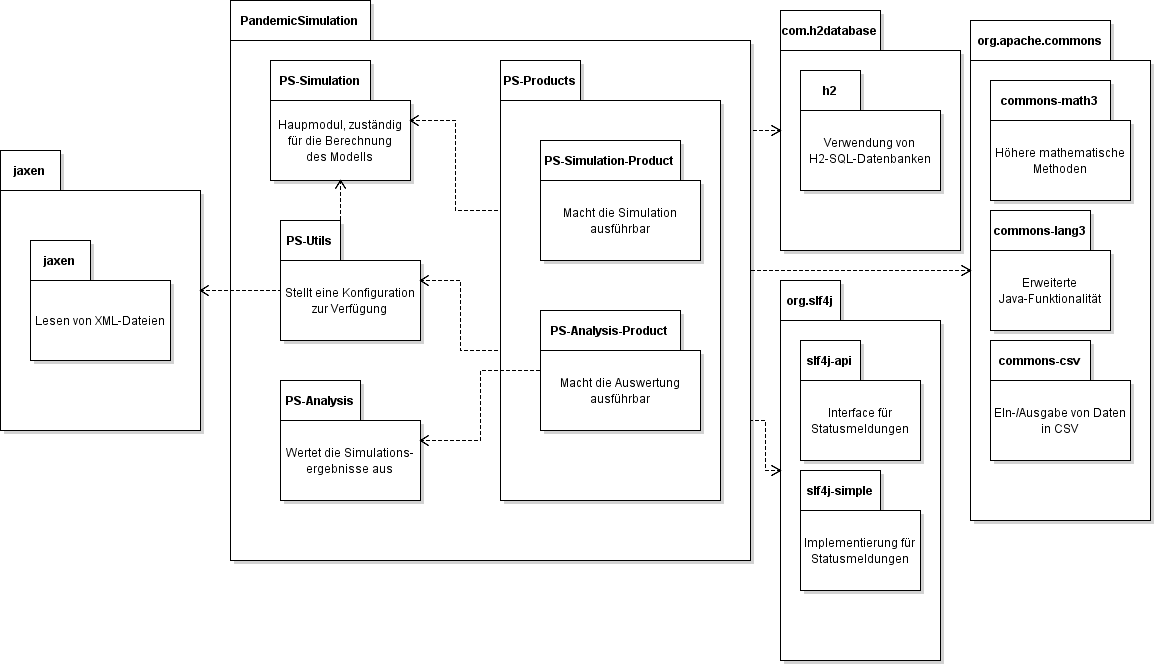
\includegraphics[width=\textwidth]{res/diagramme/Modul-Aufbau.png}
\caption{Module der Software mit externen Abhängigkeiten. Pfeile werden entlang ihrer Richtung mit ``benötigt'' gelesen.}\label{fig:ssec:sw:moduls}
\end{figure}
Die Umsetzung des in dieser Arbeit entwickelten Modells ist in dem Modul \texttt{PS-Simulation} realisiert. Der fachliche Aufbau es Moduls ist in Abbildung \ref{fig:ssec:sw:analysis} dargestellt. Um die Übersicht zu erhalten, sind die Klassen der Datenhaltung hier nicht enthalten. Grundsätzlich besitzt aber jede der hier dargestellten Klassen eine Verbindung zur Datenhaltung. Der Aufbau entspricht dem Netzwerksmodell in Abschnitt \ref{ssec:multiPop}, wobei ein \texttt{GesundheitsZustand} einem Knoten und ein \texttt{Uebergang} einer Kante entspricht. Bei letzterem wird zwischen einem Übergang zwischen zwei Gesundheitszuständen im Verlauf der Krankheit und einer Reisekante unterschieden. Um die polynomialen Volumina der Kanten abzubilden, bestehen die \texttt{InnererUebergang}-Objekte aus einem oder mehreren \texttt{UebergangsKomponente}-Objekten, wobei jedes einem Summanden entspricht.

Die Simulation läuft in diskreten Zeitschritten ab. Demzufolge wird auch von der Software jeder Zeitschritt einzeln berechnet. Die Berechnung eines solchen Zeitschrittes ist in Abbildung \ref{fig:ssec:sw:activity} veranschaulicht. Grundlage bildet wieder die Netzwerksdarstellung des Modells. Um einen deterministischen Ablauf zu gewährleisten, werden die Knoten entsprechend ihrer Identifikatoren durchlaufen. Die Kanten werden zuerst nach dem Startknoten und dann nach dem Zielknoten sortiert. Krankheitsübergänge werden vor Migrationskanten durchlaufen. Um negative Knotengrößen zu vermeiden, werden die Änderungen immer erst am Ende eines Durchlaufs übernommen. Während der Iteration werden die Änderungen zwischengespeichert. Damit wird garantiert, dass ein Knoten nicht mehr Individuen abgeben kann, als er zu Beginn der Iteration hatte.
\begin{figure}
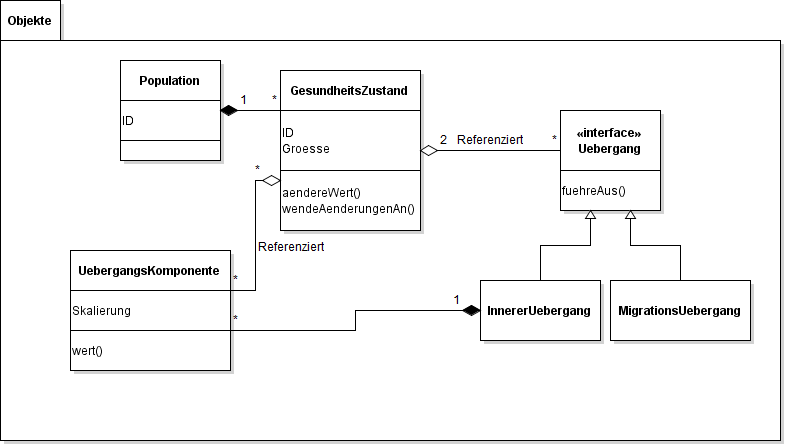
\includegraphics[width=\textwidth]{res/diagramme/Analyse-Modell.png}
\caption{Fachlicher Aufbau des Moduls \texttt{PS-Simulation} als UML-Klassendiagramm, ohne Anbindung an die Datenhaltung.}\label{fig:ssec:sw:analysis}
\end{figure}
\begin{figure}
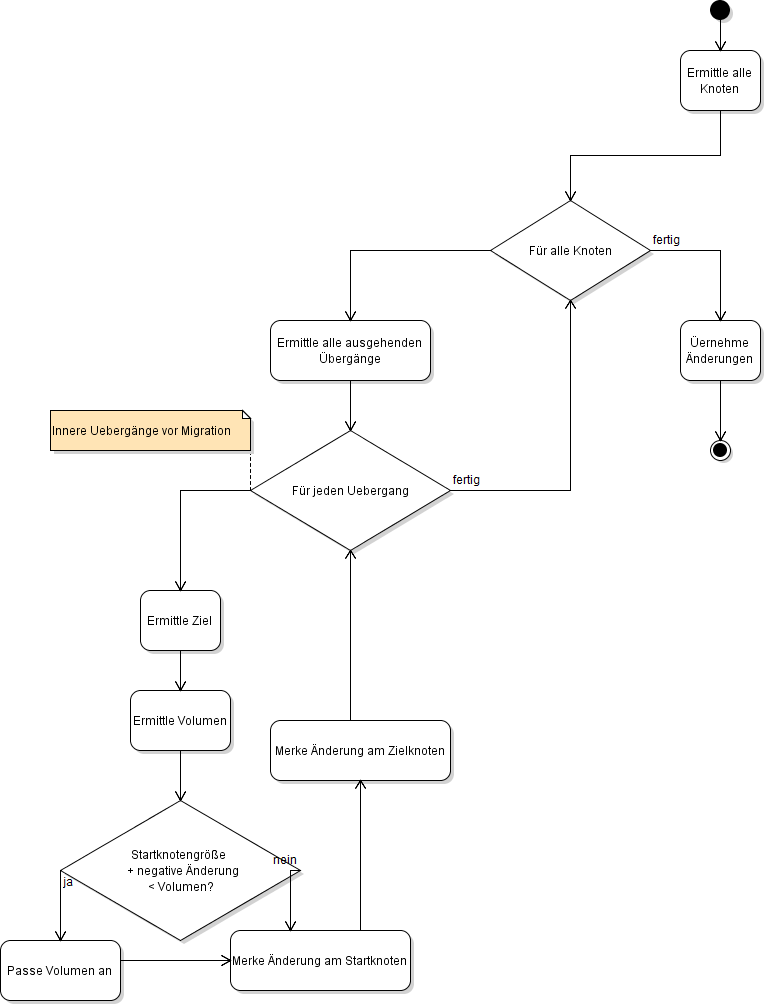
\includegraphics[width=\textwidth]{res/diagramme/Berechnung.png}
\caption{Berechnung eines Iterationsschritts als UML-Aktivitätsdiagramm}\label{fig:ssec:sw:activity}
\end{figure}
\subsubsection*{Verwendung}
Die Software wird in Form von zwei ausführbaren \texttt{jar}-Dateien bereitgestellt, deren Verwendung nachfolgend erklärt wird. Die Dateien sind über den Webdienst \emph{Github} gehostet. 


Die Datei \texttt{PS-Simulation-Product.jar} beinhaltet die eigentliche Simulationsdatei. Für die Ausführung ist der Laufzeitparameter \texttt{com.github.themetalone.pandemic.config} nötig, dessen Wert auf eine entsprechende Konfigurationsdatei zeigt. Die Konfigurationsdatei ist in XML verfasst und kennt die folgenden Elemente
\begin{description}
\item[\texttt{<simulation>}:] Das Wurzelelement der Datei. Es beinhaltet ein \texttt{<populationen>} und ein \texttt{<routen>} Element. Seine Attribute sind \begin{itemize}
	\item \texttt{datenbank}: der Pfad der zu erzeugenden Datenbank. In der vorliegenden Implementierung dient der Pfad als Prefix für die zu erzeugenden \emph{CSV}-Daten. 
	\item \texttt{zeit}: die Anzahl an Zeitschritten, die die Simulation durchlaufen soll
	\item \texttt{krankheit}: die Schwere der Krankheit, wie in Gleichung \ref{eq:ssec:multiPop:severity} beschrieben. Wird das Attribut nicht gesetzt, wird der Wert $0$ angenommen, womit der Infektionsdruck keinen Effekt mehr hat.
\end{itemize}
\item[\texttt{<populationen>}:] Ein Container für die Populationen der Definition. Beinhaltet ein \texttt{<standard>} und beliebig viele \texttt{<population>}-Elemente
\item[\texttt{<standard>}:] Die ``Blaupause'' für jede der nachfolgend definierten Populationen. Beinhaltet beliebig viele \texttt{<subpopulation>} und \texttt{<uebergang>}-Elemente. 
\item[\texttt{<subpopulation>}:] Definiert eine Subpopulation innerhalb einer Population mit folgenden Attributen:\begin{itemize}
\item \texttt{groesse}: die initiale Größe der Subpopulation. Wird das Attribut nicht angegeben, wird $0$ angenommen.
\item \texttt{name}: der Name der Subpopulation. 
\item \texttt{lebend}: gibt an, ob die Subpopulation lebende oder tote Individuen beinhaltet. Der Wertebereich ist boolesch (\texttt{true}, \texttt{false}. Wird das Attribut nicht gesetzt, wird \texttt{true} angenommen.
\item \texttt{sichtbar-infiziert}: gibt an, ob die Individuen dieser Subpopulation als infiziert wahrgenommen werden. Der Wertebereich ich boolesch. Wird das Attribut nicht gesetzt, wird \texttt{false} angenommen.
\end{itemize}
\item[\texttt{<uebergang>}:] Definiert eine Kante zwischen zwei Subpopulationen innerhalb der Population. Beinhaltet mindestens ein \texttt{<komponente>}-Element und hat die Attribute:\begin{itemize}
	\item \texttt{von}: definiert den Start der Kante. Der Wertebereich entspricht dem aller Namen von Subpopulationen.
	\item \texttt{nach}: wie \texttt{vor}, nur wird hier das Ende der Kante definiert.
\end{itemize}
\item[\texttt{<komponente>}:] Definiert einen Summanden des Kantenvolumens. Beinhaltet beliebig viele \texttt{<reference>}-Elemente und hat die Attribute:
\begin{itemize}
	\item \texttt{scalar}: ein konstanter Faktor, der auf die Größe der referenzierten Subpopulation angewandt wird. Der Wertebereich besteht aus positiven \texttt{float}-Werten.
	\item \texttt{konstante}: wenn dieses Attribute gesetzt wird, werden untergeordnete \texttt{<reference>}-Elemente sowie das \texttt{scalar}-Attribut ignoriert. Die Kante transportiert dann eine konstante Menge an Individuen pro Zeiteinheit, wie es beispielsweise für Schutzimpfungen (vgl. Abbildung \ref{fig:ssec:actions:vac}) modelliert wurde. 
\end{itemize}
\item[\texttt{<reference>}:] Referenziert die Größe einer Subpopulation. Der Wertebereich umfasst die Namen aller Subpopulationen. 
\item[\texttt{<population>}:] Definiert eine Population. Beinhaltet beliebig viele \texttt{<subpopulation>} und \texttt{<uebergang>}-Elemente. Jede Population wird mit den Informationen aus dem \texttt{<standard>}-Element initialisiert. Subpopulationen und Übergänge, die direkt in einer Population definiert werden, überschreiben Subpopulationen und Übergänge aus dem \texttt{<standard>}-Element. Ein \texttt{<population>}-Element hat folgende Attribute
\begin{itemize}
	\item \texttt{name}: der Name der Population
	\item \texttt{lebensstandard}: der Lebensstandard der Population als positiver \texttt{float}-Wert.
	\item \texttt{migrationsanteil}: der Anteil der Population, der in der Lage ist, zu migrieren. Der Wertebereich umfasst \texttt{float}-Werte im Intervall $[0,1]$.
\end{itemize}
\item[\texttt{<routen>}:] Ein Container für beliebig viele \texttt{<route>}-Elemente. \texttt{<routen>} hat die Attribute:
\begin{itemize}
	\item \texttt{reisende-subpopulationen}: definiert die Subpopulationen, deren Individuen reisen können. Der Wertebereich wird durch den Ausdruck $Subpopulation(,Subpopulation)^*$ beschrieben (Beispiel: \texttt{S,E}). 
	\item \textbf{flugverkehr}: definiert, ob ein Flugverkehrsnetz automatisch generiert werden soll. Der Wertebereich ist boolesch. Falls das Attribut nicht gesetzt wird, wird \texttt{false} angenommen. Bei \texttt{true} wird eine zusätzliche Reisekante zwischen den reisenden Subpopulationen aller Populationen erzeugt. Die Kanten werden als Flugrouten gekennzeichnet. Der Anteil am noch nicht zugewiesenen Migrationsanteil einer Population wird gleichmäßig auf die neu erzeugten Kanten verteilt. Wird für die Population bereits eine Flugroute definiert, wird bei der automatischen Generierung diese Flugroute ausgelassen. 
\end{itemize}
\item[\texttt{<route>}:] Definiert eine unidirektionale Route zwischen zwei Populationen. Dadurch werden Reisekanten zwischen den reisenden Subpopulationen der verbundenen Populationen erzeugt. Ein \texttt{<route>}-Element besteht aus beliebig vielen \texttt{<zuordnung>}-Elementen und hat die Attribute:\begin{itemize}
	\item \texttt{von}: die Startpopulation, angegeben durch ihren Namen.
	\item \texttt{nach}: die Zielpopulation, angegeben durch ihren Namen.
	\item \texttt{flug}: gibt an, ob eine Route eine Flugroute ist, oder nicht. Der Wertebereich ist boolesch. Wird das Attribut nicht gesetzt, wird \texttt{false} angenommen.
	\item \texttt{anteil}: der Anteil der Route am Migrationsanteil. Der Wertebereich sind \texttt{float}-Werte im Intervall $[0,1]$. Wenn das Attribut nicht gesetzt wird, wird $1$ angenommen.
\end{itemize}
\item[\texttt{<zuordnung>}:] Definiert eine manuelle Reisekante zwischen Subpopulationen verschiedener Populationen. Wird ein \texttt{<zuordnung>}-Element gesetzt, muss die Route vollständig durch Zuordnungen definiert werden. Ein \texttt{<zuordnung>}-Element hat die folgenden Attribute:\begin{itemize}
	\item \texttt{vonSubpopulation}: referenziert eine Subpopulation in der Ausgangspopulation. Der Wertebereich besteht aus den Namen der dort existenten Subpopulationen. 
	\item \texttt{nachSubpopulation}: referenziert eine Subpopulation in der Zielpopulation. Der Wertebereich ist analog zu dem von \texttt{vonSubpopulation}
\end{itemize} 
\end{description}

\subsubsection*{Lizenzen}